\documentclass[12pt,a4paper,final]{report}
\usepackage[utf8]{inputenc}
\usepackage{amsmath}
\usepackage{amsfonts}
\usepackage{amssymb}
\usepackage{longtable}
\usepackage{gensymb}
\usepackage{eurosym}
\usepackage{fixltx2e}
\usepackage{caption}
\usepackage{float}


% ----------------------------------------------
% Bibliography
% ----------------------------------------------
\usepackage[autostyle]{csquotes}
\usepackage[
backend=biber,
hyperref=true,
style=numeric,
sorting=none,
autocite=plain
]{biblatex}
\addbibresource{final_thesis.bib}

\usepackage{hyperref}
\hypersetup{
colorlinks=true,
linkcolor=black,
citecolor=black,
urlcolor=blue
}

% ----------------------------------------------
% Images
% ----------------------------------------------
\usepackage{wrapfig}
\usepackage{graphicx}
\usepackage{float}
\floatstyle{boxed}
\graphicspath{ {figures/} }
%\restylefloat{figure}
\newcommand*{\captionsource}[2]{%
  \caption[{#1}]{%
    #1%
    \\\hspace{\linewidth}%
    Source: #2%
  }%
}

% ----------------------------------------------
% Code blocks
% ----------------------------------------------
\usepackage{listings}
\usepackage{color}
\usepackage{courier}

\definecolor{dkgreen}{rgb}{0,0.6,0}
\definecolor{gray}{rgb}{0.5,0.5,0.5}
\definecolor{mauve}{rgb}{0.58,0,0.82}

\lstset{ %
basicstyle=\footnotesize\ttfamily,
numbers=left,
numberstyle=\footnotesize\color{gray},
stepnumber=1,
numbersep=5pt,
backgroundcolor=\color{white},
commentstyle=\color{dkgreen},
keywordstyle=\color{blue},
stringstyle=\color{mauve},
rulecolor=\color{black}, 
showspaces=false,
showstringspaces=false,
showtabs=false,  
frame=single,
tabsize=2, 
captionpos=b,
breaklines=true, 
breakatwhitespace=false,  
escapeinside={\%*}{*)} 
}

% ----------------------------------------------
% Title styling
% ----------------------------------------------
\usepackage{titlesec}

\titleclass{\part}{top}
\titleformat{\part}[display]{\centering\normalfont\Huge\bfseries}{\titlerule[5pt]\vspace{3pt}\titlerule[2pt]\vspace{3pt}\MakeUppercase{\partname} \thepart}{0pt}{\titlerule[2pt]\vspace{1pc}\huge}
\titlespacing*{\part}{0pt}{0pt}{20pt}

\titleclass{\chapter}{straight}
\titleformat{\chapter}[hang]
{\normalfont\Large\bfseries}{\thechapter} {0.5em}{} 
\titlespacing*{\chapter}{0pt}{0pt}{0pt}

\titleclass{\section}{straight}
\titleformat{\section}[hang]
{\normalfont\large\bfseries}{\thesection} {0.5em}{} 
\titlespacing*{\section}{0pt}{0pt}{0pt}

% ----------------------------------------------
% Paragraph styling
% ----------------------------------------------
\setlength{\parindent}{0pt}
\setlength{\parskip}{1ex plus 0.5ex minus 0.2ex}

\title{WTherm - Web-connected smart thermostat}
\author{Niek Blankers}

\begin{document}
\begin{titlepage}
% ----------------------------------------------
% Title page
% Downloaded from http://www.LaTeXTemplates.com
% License:
% CC BY-NC-SA 3.0 (http://creativecommons.org/licenses/by-nc-sa/3.0/)
% ----------------------------------------------
\newcommand{\HRule}{\rule{\linewidth}{0.5mm}}

\center

\textsc{\LARGE Final Thesis}\\[1.5cm]

\HRule \\[0.4cm]
{ \huge \bfseries WTherm}\\[0.4cm]
\textsc{\large Web-connected smart thermostat}\\[0.2cm]
\HRule \\[3.5cm]

\begin{minipage}{0.4\textwidth}
\begin{flushleft} \large
\emph{Author:}\\
Niek \textsc{Blankers} (A6b)
\end{flushleft}
\end{minipage}
~
\begin{minipage}{0.4\textwidth}
\begin{flushright} \large
\emph{Supervisor:} \\
Dolf \textsc{Breederveld}
\end{flushright}
\end{minipage}\\[8cm]

{\large \today}\\[0.3cm] 
\begin{figure*}[!b]
	\centering
	\hyperref[chap:License]{
\includegraphics{by-nc-sa}}
\end{figure*}

\vfill

\end{titlepage}

\begin{abstract}
This thesis delineates the research and design process involved in the develop\-ment of the WTherm, a smart thermostat. The thermostat was installed in a single household. A thermal model of the living room in question is used to calculate the amount of time until a certain target temperature will be reached. This calculation is used to start heating at exactly the right time to reach the targets defined in a schedule that's programmable through a web interface. As a result, the WTherm saves a considerable amount of energy in comparison to a traditional room thermostat. 

The calculated savings over the course of a single winter in this particular case exceed \EUR{16}. This means that the WTherm will have paid for itself within three years.
\end{abstract}

\setcounter{tocdepth}{1}
\tableofcontents

\part*{Preamble}
\phantomsection
\addcontentsline{toc}{part}{Preamble}
The inspiration for this project originated from my father's request to develop a basic thermostat he could remotely program through a web interface. After a couple of weeks of research and development, this thermostat was installed in his house and dubbed the WTherm alpha project\footnote{\url{https://github.com/NiekProductions/WTherm-alpha/}}. 

After installing the Nest smart thermostat\footnote{\url{https://nest.com/}} in my mother's house, I decided to revisit the WTherm project and to try to develop it further into a smart thermostat.

I am very thankful to Mr. Breederveld and Albert Vos, as I greatly appreciate their assistance over the course of this project.
I would also like to thank the LeMaker\footnote{\url{http://www.lemaker.org/}} team for donating a Banana Pi after reading my research plan.
\newpage

\part*{Introduction}
\phantomsection
\addcontentsline{toc}{part}{Introduction}
In practically every house with a central heating system you will find a thermostat. The very first electric thermostat (or "temperature regulator") was patented in 1893 by Albert Butz. It described a bimetallic strip that, when bent by a decrease in temperature, would make electrical contact and power a motor which would in turn adjust the dampers of a furnace\cite{Butz1893Temperature}.

Butz's invention was revolutionary, but it lacked a feature before making it into the households of many. Nowadays, most thermostats feature a programmable schedule which can be used to set daily times at which the heating should turn on.

A recent development in the field of central heating control has been the introduction of smart thermostats. These thermostats offer Wi-Fi or wired connectivity for remote control and claim to improve energy efficiency. Being one of the first smart thermostats on the market in 2011, the Nest thermostat\footnote{\url{https://nest.com/}} aims to save energy by learning when a user leaves the house and automatically turning off the heater. The Nest Thermostat also learns the time required to heat up the house in order to show the amount of time necessary to reach the temperature desired by the user\cite{NestInsideOut}.

Heating a house consumes a substantial amount of energy. The speed at which a central heating system can heat up a room varies on a day-to-day basis. If the time during which the central heating is on can be reduced by even half an hour every day, a significant amount of the annual energy usage can be saved. This is the approach to energy conservation used in this project.

\chapter*{Research objective} \label{chap:ResearchObjective}
The objective of this project is to design and develop a smart thermostat that saves heat by predicting or calculating the time it takes a room to heat up to a certain temperature. The thermostat must use this calculation to precisely follow a weekly schedule that can be programmed through a web interface. The scope of this project will be limited to a single situation in which a district heating unit is used to heat a living room.

The following research topics can be distilled from the main objective:
\begin{itemize}
	\item How can the heating time be predicted?
	\item What hardware and software is necessary to run the thermostat?
	\item How can a web interface be implemented?
	\item What safety features are required?
	\item How much energy does this solution save compared to a traditional room thermostat?
\end{itemize}

Additionally, the user interface needs to meet the following demands:
\begin{itemize}
	\item A secure implementation of a login system for user authentication.
	\item The option to program a weekly schedule.
	\item The option to set a manual temperature that overrides the schedule.
	\item A page to view past temperatures through charts.
	\item A page to change user data.
\end{itemize}

\chapter*{Hypothesis}
The hypothesis is that the WTherm saves heat in comparison with a clock thermostat set to start heating at a fixed time every morning.

\chapter*{Project summary}
The first step to meet the aforementioned objective is to find a way to predict the time it will take the temperature of the living room to meet a target. This process is described in part~\ref{part:PredictHeatingTime}. In the first chapter, heat flow is explained through formulas. In the second chapter these formulas are applied to the situation and used to form a thermal model of the living room. This model is also verified and a way is described in which the model can be used to predict the time it will take the temperature in the living room to reach a certain level, solving the first part of the research objective.
 
Part~\ref{part:ConstructThermostat} of this thesis deals with the construction of the thermostat. The necessary hardware and software to run the thermostat is discussed. 

The database structure and interaction and the way passwords are securely stored is reviewed in chapters \ref{chap:databaseStructure} to \ref{chap:passwordHashing}, while chapters \ref{chap:readTempSensors} and \ref{chap:heaterInterface} deal with the hardware level of the thermostat.

Chapters \ref{chap:layout} and \ref{chap:codeOverview} give an overview of the code that runs the WTherm and its web interface, as well as an insight into the function of each file in the source code. Finally, the implemented safety features are discussed in chapter~\ref{chap:safety}.
 
In part~\ref{part:CalculateSavings} of this thesis the hypothesis is tested by comparing the WTherm to a traditional clock thermostat over the course of a single week in the winter.

\part{Predicting the heating time} \label{part:PredictHeatingTime}
This part describes how to calculate the amount of time it will take to heat up the room to a certain temperature. In the first chapter, the formulas describing how heat flows in a system will be explained. Next, these formulas will be applied to the situation in question and they will be used to form a thermal model of the living room that can then be used in the thermostat to determine when to start heating.

\chapter{Thermal calculations}
Heat capacity (or thermal capacity) is a constant that describes the ratio between thermal energy and temperature.It is expressed in Joules per Kelvin, indicating the amount of heat that results in a temperature change of a single Kelvin or degree Celsius\cite{chemwiki14}. Calculation of the heat capacity is done using the following formula:
\begin{equation} \label{eq:ThermalCapacity}
C = \frac{Q}{T}
\end{equation}
With $C$ being the heat capacity in Joule per Kelvin, $Q$ the added thermal energy in Joules and $T$ the difference in temperature in Kelvin or degrees Celsius.

However, the heat capacity determined by the above-mentioned formula can only be used in a system where heat cannot be transferred away from the system. In practice, this is highly unlikely to occur since perfect isolation on a small scale is impossible. The heat that is transferred away needs to be taken into account. Heat can be transferred in three ways:
\begin{itemize}
	\item Conduction
	\item Convection
	\item Radiation
\end{itemize}
Conduction is heat transfer inside a material. Heat flows from particles with more kinetic energy to particles with less kinetic energy\cite{Hyperphysics98}. Heat transfer through conduction can be described in a linear formula as follows:

\begin{equation} \label{eq:HeatConduction}
P = A\cdot U\cdot (T_{i}-T_{o})
\end{equation}

\textit{P} being the conducted power in Watts, \textit{A} the surface area in $\mathrm{m^{2}}$ of the material through which the heat is conducted, \textit{U} the heat transfer coefficient in $W/(m^{2}K)$ and $(T_{i}-T_{o})$ the difference between inside and outside temperature\cite{thermopedia11}.

\textit{"Convection is heat transfer by mass motion of a fluid such as air or water when the heated fluid is caused to move away from the source of heat, carrying energy with it."}\cite{Hyperphysics98}. Inside for example a system with a heat source and a medium, this would be the medium that expands and changes in density as it's heating, causing a flow that transports energy.

Heat transfer through radiation is caused by electromagnetic waves, most of which are in the infrared region. According to the Stefan-Boltzmann law\cite{engineeringtoolbox14}, radiated heat uses the form:

\begin{equation} \label{eq:HeatRadiation}
Q = A\cdot \sigma \cdot{} T^{4} \cdot{} t
\end{equation}

In this formula, $Q$ is the transferred heat in Joules, $\sigma$ the Stefan-Boltzmann constant ($\mathrm{5,6703\times 10^{-8} W/m^{2}K^{4}}$ in the case of a blackbody, less depending on the material), $A$ the area in $\mathrm{m^{2}}$, $T$ the absolute temperature in Kelvin and $t$ the total time in seconds.

This concludes the description of the formulas that will be used in the specific situation set out in the next chapter.

\chapter{Creating the thermal model of the room} \label{chap:createModel}
The previous chapter introduced the formulas that describe the thermal energy in a system and the heat flow in and out of the system. In this chapter, these formulas will be applied to the situation in question, in this case a living room. Three manners of heat flow were described, namely conduction, radiation and convection. Since the living room is mostly isolated against convection to the outside, the effect of convection will not be noticeable. Radiation only significantly occurs at very high temperatures, so it is also out of the question. 

Conduction is the only important form of heat transfer in this case. This means that the heat flowing out of the living room can be described in a formula similar to~\eqref{eq:HeatConduction}, replacing the area and U-value with an overall heat transfer coefficient $C_{transfer}$ (or $C_{t}$) in W/K: 

\begin{equation} \label{eq:Ctransfer}
C_{t} = \frac{P}{dT} = \frac{P}{T_{i}-T_{o}} \quad \text{provided that $\mathrm{dT\neq{}0}$}
\end{equation}

The First Law of Thermodynamics states that energy is saved; it can be neither created nor destroyed\cite{Bodner1stTherm}. According to this principle, one can deduce that when \textit{x} amount of heat is added to a system and \textit{y} amount escapes, the amount of heat left in the system is \textit{x-y}. If the thermal profile of the system is considered according to this principle, one can state that the heat contained in the room is equal to the difference between the total heat added by the heating system and the heat loss:

\begin{equation} \label{eq:QheatDiff}
Q_{heat} = Q_{in} - Q_{loss}
\end{equation}

$Q_{loss}$ can be calculated from the $C_{t}$ value \eqref{eq:Ctransfer} and $Q_{in}$ from the central heating power. The U value in W/K can be determined by keeping the room at a certain temperature and measuring the required power. This temperature has to exceed the outside temperature as the amount of heat flowing into the room can't easily be measured. If the thermal profile is considered in time steps of $dt$ and temperature steps of $dT$, one can state that:

\begin{equation} \label{eq:Qheat}
Q_{heat} = C\cdot dT
\end{equation}
\begin{equation} \label{eq:Qin}
Q_{in} = P\cdot dt
\end{equation}
\begin{equation} \label{eq:Qloss}
Q_{loss} = C_{t}(T-T_{o})\cdot dt
\end{equation}


Now according to \eqref{eq:QheatDiff} through \eqref{eq:Qloss} one can form a differential equation as follows:
\begin{equation} \label{eq:diffEq}
\frac{dT}{dt} = \frac{P-C_{t}(T-T_{o})}{C}
\end{equation}

This differential equation contains a linear component, making it unpractical to solve. A better approach would be to create a model. The term 'model' refers to a simplified version of the target system, including only the relevant aspects.\cite{ModelsInPhysics} The thermal model will create the temperature curve by repetitively calculating $dT$ for small steps of $dt$. $dT$ can be defined as: 

\begin{equation} \label{eq:dT}
dT = \frac{Q_{in}-Q_{loss}}{C} = \frac{P\cdot dt -C_{t}(T-T_{o})\cdot dt}{C}
\end{equation}

With $Q_{in}$ and $Q_{loss}$ being defined in \eqref{eq:Qin} and \eqref{eq:Qloss} on page \pageref{eq:Qloss}. The temperature curve can then be calculated:
\lstset{language=Python}
\begin{lstlisting}[caption={(pseudocode) calculating the temperature curve},label={lst:tempCurve}]
# Starting values
t = 0 s
dT = 0 K
T = .. degC 
To = .. degC

# Constants
Ct = .. W/K
P = .. W
C = .. J/K
dt = 60 s
t_max = 3600 s

# Loop
while t < t_max:
	Qin = P * dt
	Qloss = Ct * (T-To) * dt
	dT = (Qin - Qloss)/C
	T = T + dT
	t = t + dt
\end{lstlisting}

In conclusion, the constants that need to be determined to create the thermal model are:
\begin{description} \label{variableDesc}
	\item[P] The heating power in Watts
	\item[$\mathbf{C_{t}}$] The heat transfer coefficient in W/K
	\item[C] The room's heat capacity
\end{description}

\section{Calculating P, C\textsubscript{t} and C} \label{sec:CalculatePUC}
To complete the thermal model described in the previous section, the heating power, heat transfer coefficient and the heat capacity will need to be determined. This will be done according to a single measurement, where the room will first be heated up to 19.5\degree{}C and then maintained at this temperature by a traditional room thermostat.

Calculating the heating power is fairly simple. The heater will constantly be powered on when the temperature hasn't reached the target of 19.5\degree{}C yet, so if the time it takes to heat up as well as the heat spent in this time are measured they can be used to calculate the average heating power.

The heat transfer coefficient $C_{t}$ will be calculated from the measurements when the temperature has already reached the target. According to \eqref{eq:QheatDiff}, if $Q_{heat}$ remains constant, the added heat $Q_{in}$ is equal to the lost heat $Q_{loss}$. Any heat spent to keep the room temperature constant is heat that's being conducted out of the room. The added energy divided by the amount of time during which the temperature is kept constant will result in the total power used in Watts. Divide this by the difference in inside and outside temperature following \eqref{eq:Ctransfer} and the resulting constant is $C_{t}$.

$C_{t}$ can then be used to calculate the heat capacity $C$. For every interval between measurements, the lost heat $Q_{loss}$ is determined by multiplying $C_{t}$ by the difference between the inside and outside temperature. The total added heat $Q_{in}$ can then be subtracted by this heat loss, resulting in the net added heat $Q_{net}$. The heat capacity $C$ is equal to the net heat used to increase the room temperature divided by the total temperature rise conforming \eqref{eq:ThermalCapacity}.

In conclusion, to actually create the thermal model, it is first of all necessary to calculate the heating power \textit{P}, heat transfer coefficient $C_{t}$ and heat capacity $C$. The room will be heated to 19,5\degree{}C and kept at that temperature for several hours. The added heat will be measured, as well as the inside and outside temperatures.

\subsection{Reading added heat from the heat meter}
To create a model of the temperature in the living room, a way to measure the heat added to the system is necessary. The central heating consists of a district heat exchange unit with an external heat meter. 

\begin{wrapfigure}{r}{0.3\textwidth}
  \vspace{-33pt}
  \begin{center}
      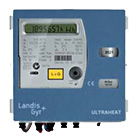
\includegraphics[width=0.28\textwidth]{2WR5}
  \end{center}
  \vspace{-20pt}
  \captionsource{2WR5 heat meter}{\url{tls.se}}
\end{wrapfigure}
The heat meter is a Landis \& Gyr Ultraheat 2WR5. The 2WR5 can be read out directly from the LCD display, which displays the accumulated quantity of thermal energy in gigajoules with three decimal numbers. 0,001 GJ is equal to 1 MJ, which is the same as 3,6\textsuperscript{-1} kilowatt hours, or about 278 Wh.

To log the added heat, an IP camera\footnote{A security camera connected to the network} was mounted directly in front of the heat meter, with a small light next to it illuminating the screen. A snapshot can be fetched by sending a request to a HTTP URL, in this case \url{http://<camera-IP>/snapshot.cgi}. A shell script was used to run on a remote linux machine every five minutes:
\lstset{language=bash}
\begin{lstlisting}[caption={Downloading and renaming a snapshot}]
#!/bin/sh
wget http://<camera-IP>/snapshot.cgi --user=admin --password=password -O snaps/snapshot-`date +%Y-%m-%d-%H%M%S`.jpg -T 60
\end{lstlisting}
This script resulted in pictures like figure~\ref{fig:snap}, which were subsequently copied into a spreadsheet.
\begin{figure}[H] 
  \begin{center} 
      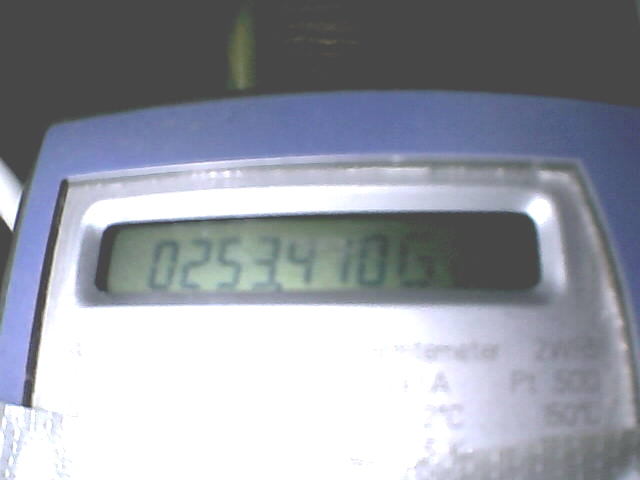
\includegraphics[width=0.75\textwidth]{snapshot-2014-12-13-060001}
  \end{center}
  \caption{Sample picture from IP camera}
  \label{fig:snap}
\end{figure} 

\subsection{Temperature readings} \label{sec:TempReadings}
Temperature measurements from inside and outside the living room are also needed. The house already has two wireless temperature sensors installed. One is located in the living room, while the other is outside of the house. These sensors are connected to a 
Homewizard\footnote{\url{http://www.homewizard.nl/}}, an internet-connected smart-home device which can be accessed by requesting different URLs. To obtain the inside and outside temperature, an HTTP request is made to \url{http://<homewizard-IP>/<password>/telist}\cite{HomeWizardAPI}. The WTherm alpha project was used in this case, as it already logs the inside and outside temperatures every five minutes. The MySQL database containing the measurements was later exported into a spreadsheet.

\subsection{Obtained measurements}
A graph of the data obtained from the heat meter and temperature sensors looks like this:
\begin{figure}[H]
  \begin{center}
      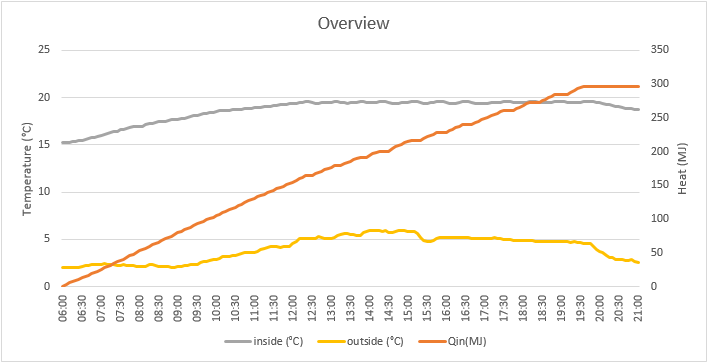
\includegraphics[width=0.95\textwidth]{GraphMeasurements}
  \end{center}
  \caption{Raw temperature/heat measurements}
\end{figure}
Between 06:00 and 12:00, the room was heated from 15,3\degree{}C to 19,5\degree{}C. This temperature was maintained until 19:30.

The total energy used while heating up is 155MJ. Converting this to kWh and dividing it by 6 hours results in an average heating power $P$ of 7,2kW.

Keeping the room at 19,5\degree{}C from 12:30 to 19:30 required 36,39kWh, or 5,2kW. The average difference in inside and outside temperature. Following \eqref{eq:Ctransfer}, the heat transfer coefficient $C_{t}$ ends up at approximately 364 W/K.

\begin{figure}[H]
  \begin{center}
      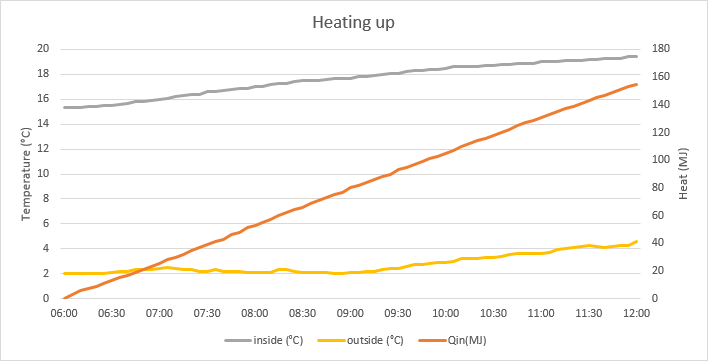
\includegraphics[width=0.95\textwidth]{GraphHeatingMeasurements}
  \end{center}
  \caption{Measurements while heating}
\end{figure}
Using $C_{t}$, the amount of heat lost in every five minute interval between measurements can be calculated. Subtracting the added heat by the lost heat as described at the start of this section on page~\pageref{sec:CalculatePUC} results in $Q_{net}$:
\begin{figure}[H]
  \begin{center}
      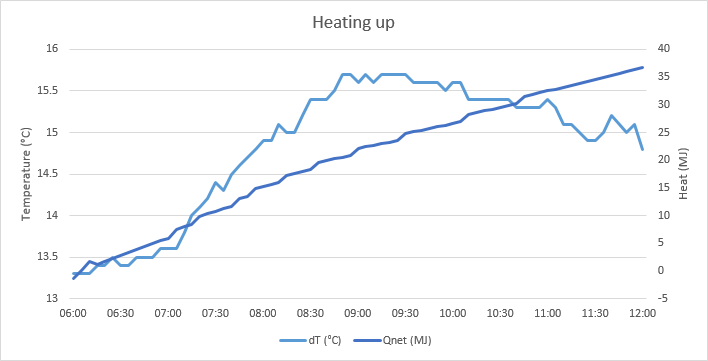
\includegraphics[width=0.95\textwidth]{GraphHeatingMeasurements-calculated}
  \end{center}
  \caption{Calculated $Q_{net}$ and $dT$}
\end{figure}
The net added heat when heating up was roughly 37MJ. Dividing this by the temperature rise of 4,1\degree{}C according to \eqref{eq:ThermalCapacity} results in a heat capacity $C$ of about $8,978\times 10^{6}$ J/K. 
All of the measurements and calculations can be found on GitHub using the link found on page~\pageref{chap:Software}.

The necessary constants for the model listed on page~\pageref{variableDesc} have now been determined. In the next section, the resulting model will be verified against the measurements.

\section{Verifying the thermal model}
To validate this model, it can be compared to the measurements. Since the heating time has to be predicted, the outside temperature is assumed to be constant. In this case, an average outside temperature of 2,75\degree{}C during the measurements is used. The starting temperature $T$ is 15,3\degree{}C. The following graph was drawn using the code from listing~\ref{lst:tempCurve}. A $dt$ of 5 minutes and a total time of 6 hours was used:
\begin{figure}[H]
  \begin{center}
      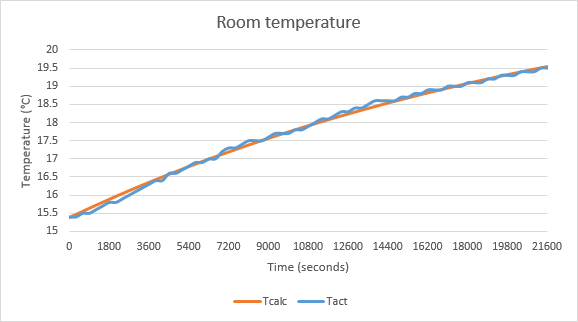
\includegraphics[width=0.95\textwidth]{GraphModelTest-compare}
  \end{center}
  \caption{Testing the temperature model with the measurements superimposed.}
\end{figure}
$Tcalc$ in this chart is the temperature as calculated by the model, and $Tact$ the actual measured temperature for comparison. The calculated temperature reaches a maximum of 19.5\degree{}C, which corresponds with the temperature measured after 6 hours.

\section{Using the thermal model} \label{sec:usingModel}
In the previous sections, the model was determined and tested to match to the actual situation. Using this model to predict the time it takes the temperature to reach a certain target can be done using a while loop that steps through the model for intervals of $dt$. The following code is an adaptation of listing~\ref{lst:tempCurve} from page~\pageref{lst:tempCurve} that can be used in the thermostat:
\lstset{language=Python}
\begin{lstlisting}[caption={(pseudocode) calculating the heating time from 15 to 20 degrees with a constant outside temperature of 5 degrees}]
# Starting values
t = 0 s
dT = 0 K
T = 15 degC 
Target = 20 degC
To = 5 degC

# Constants
Ct = 364 W/K
P = 7176 W
C = 8978053 J/K
dt = 60 s

While T < Target:
	Qin = P * dt
	Qloss = Ct * (T-To) * dt
	dT = (Qin - Qloss)/C
	T = T + dT
	t = t + dt

Required time = t
\end{lstlisting}
Now that the model has been created and approved, the next part will describe how it was integrated into the thermostat.

\part{Constructing the thermostat} \label{part:ConstructThermostat}
This part will describe how the thermostat itself was constructed. First the hardware choice will be justified.
\chapter{Hardware choice} \label{chap:HardwareChoice}
Three hardware platforms were considered to run the thermostat, namely:
\begin{itemize}
  \item Arduino
  \item Raspberry Pi
  \item Banana Pi
\end{itemize}
\section*{Arduino Uno}
\begin{wrapfigure}{r}{0.3\textwidth}
  \vspace{-33pt}
  \begin{center}
      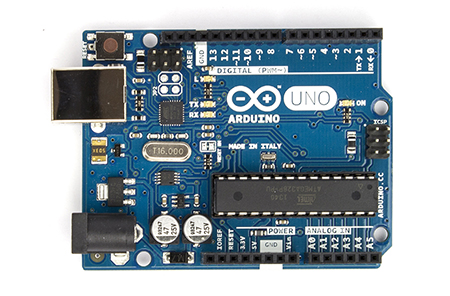
\includegraphics[width=0.28\textwidth]{arduinounor3}
  \end{center}
  \vspace{-20pt}
  \captionsource{Arduino Uno}{\url{arduino.cc}}
\end{wrapfigure}
The Arduino Uno is an open-source microcontroller platform developed by the Italian Arduino company. It comes with an easy-to-use IDE for writing software for the board. The board features an 8-bit Atmel ATmega328p microprocessor running at 16 MHz with 32 kilobytes of programmable flash, 1K of EEPROM, 2K of SRAM and 23 I/O lines, of which 6 are PWM channels and 6 are ADC inputs\cite{atmega328p}. The Arduino is programmed using C++ from the Wiring-based IDE, with a number of code libraries to simplify programming\cite{arduinounorev3}.

A very early prototype of the WTherm alpha was run on an Arduino. The Arduino doesn't have built in networking, so an external Ethernet module was connected. Since no TCP stack was already built into the Arduino, the networking had to be programmed on a very low level. Combined with the limited memory available this makes it unsuitable to run a reasonable website and database. The Arduino is great for direct low-level access to hardware, but the disadvantages outweigh this advantages which is why I chose not to run the thermostat on an Arduino.
\newpage
\section*{Raspberry Pi}
\begin{wrapfigure}{r}{0.3\textwidth}
  \vspace{-33pt}
  \begin{center}
      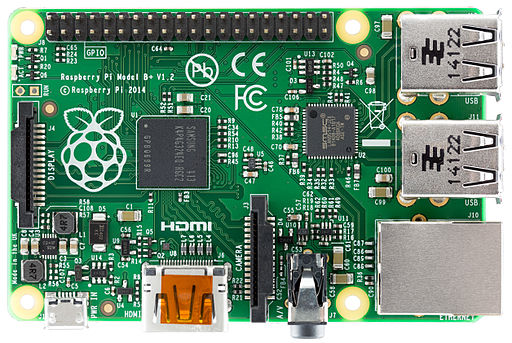
\includegraphics[width=0.28\textwidth]{RaspberryPiTop}
  \end{center}
  \vspace{-20pt}
  \captionsource{Raspberry Pi}{\url{wikimedia.org}}
\end{wrapfigure}

The Raspberry Pi is a very popular low cost credit-card sized computer. It's based around a 700MHz ARMv6 processor with 500MB of RAM. It features on-board networking, GPIO, video output, USB and a low power consumption. The Raspberry Pi is able to run a variety of linux distributions, including debian and fedora\cite{RasPiDoc}.

The Raspberry Pi almost meets the demands. It can run a web server and it has built-in networking. It does however run off an SD card. The many read/write-operations of a the database can cause the flash storage in an SD card to become corrupted, which is an issue that I encountered in the WTherm alpha project.

\section*{Banana Pi}
\begin{wrapfigure}{r}{0.3\textwidth}
  \vspace{-33pt}
  \begin{center}
      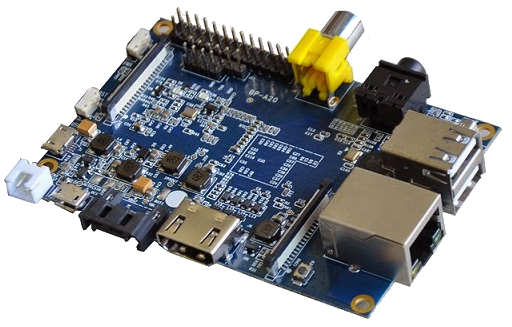
\includegraphics[width=0.28\textwidth]{BananaPi}
  \end{center}
  \vspace{-20pt}
  \captionsource{Banana Pi}{\url{bananapi.org}}
\end{wrapfigure}
The Banana Pi is a hardware platform similar to the Raspberry Pi. Instead of a single-core ARMv6 processor, it uses a dual-core ARMv7 running at 1 GHz with 1GB of RAM. This increase in processing power results in higher web server performance. In addition to GPIO, USB and networkingit also has a Serial ATA connector. This means that it's able to run off an external hard drive, making it more suitable for running a database\cite{BananaPiDoc}. This is why I chose the Banana Pi for this project.

\chapter{Web server}
Now that the hardware choice has been made, the next step is to choose a web server to run the code on.
\section*{Apache}
Apache is a very popular open-source web server that runs on nearly every modern operating system. Apache has played a key role in the early development and growth of the World Wide Web. \cite{ApacheServer}.

Apache is a process-based server. This means that it has to spawn new processes for each task, making it very CPU and memory-intensive. Since the hardware platform for this application has a limited amount of memory and processing power, Apache would not perform very well\cite{WikiVSApacheNginx}.
\section*{Nginx}
Nginx (pronounced "engine-x"), just like Apache, is a free, open-source web server. \textit{"Nginx is known for its high performance, stability, rich feature set, simple configuration, and low resource consumption."}\cite{nginxWiki}

Unlike Apache, nginx is an event-based web server. It operates asynchronously, and handles requests in a low number of threads. Nginx consumes less RAM than Apache, has better caching and serves web pages more quickly\cite{WikiVSApacheNginx}. This is why nginx was chosen to run the thermostat.

\chapter{Programming language}
Now that the hardware platform and the web server have been chosen, all that's left is to choose a programming language. In this chapter, two languages will be compared: Python and PHP.
\section*{Python}
Python is a widely used open source high-level language that's supported by large developer communities. It uses strict indentation enforcement and aims to be the most readable programming language. Since the Python interpreter supports modules and packages, only the necessary modules have to be imported. This results in less runtime than comparable code in a different programming language.\cite{WhatIsPython}

\section*{PHP}
The WTherm alpha project's source code was written in PHP. Much like Python, PHP\footnote{a recursive acronym for "PHP: Hypertext Preprocessor"} is an open-source, interpreted, high level language. It is especially suited for web development. PHP is a server-side language, which means that the code is executed on a server, generating output (normally HTML) which is then sent to the client. Unlike the case with the client-side language Javascript, the client only ever gets to see the code's output, not the underlying code itself. PHP is a very simple language, which is why it's excellent for beginners\cite{PHPintro}. Because of my previous experience and knowledge with PHP, it's used for this project.

\chapter{Database structure} \label{chap:databaseStructure}
The thermostat will be running from a MySQL database. MySQL is an open-source relational database management system. It uses SQL\footnote{Structured Query Language} to manage data\cite{WhatIsMySQL}. This chapter will describe the database structure.

\section*{Status}
Since the thermostat script will run every 5 minutes, a status table in the database is used to store the last measurements and state. This means that the user interface can request the last measurements without having to obtain direct access to the sensor outputs. This table consists of the following columns:
\begin{description} \label{statusCols}
	\item[T] Float -  The inside temperature
	\item[T\_o] Float - The outside temperature
	\item[T\_target] Float -  The target temperature
	\item[Heating] Boolean - Whether the heater is on
	\item[Override] Boolean - Whether manual temperature is enabled
	\item[Last\_update] Timestamp - The last time the script has successfully ran
\end{description}
Now the most recent measurements and status are stored in a central table, accessible to both the thermostat script and the client web interface.

\section*{Schedule}
The thermostat will need a schedule, containing the target temperatures and the time/day when this temperature needs to be reached. Since the thermostat uses a weekly schedule, the table structure reads as follows:
\begin{description} \label{scheduleCols}
	\item[T\_target] Float - The target temperature
	\item[time] Varchar - The time (00:00-23:59)
	\item[day] Integer - The weekday (1-7)
\end{description}
A primary key constraint between \textbf{time} and \textbf{day} was set up to prevent duplicate entries.

\section*{Log}
This table is used to store measurements, which can be used 
\begin{description} \label{logCols}
	\item[Time] Timestamp - The time
	\item[T] Float - The inside temperature
	\item[T\_target] Float - The target temperature
	\item[T\_o] Float - The outside temperature
	\item[Heating] Boolean - Whether the heater is on
\end{description}
The \textbf{Time} column is made a primary key to prevent duplicate entries.

\section*{Users}
This database table is used to store login users and their password hashes.
\begin{description} \label{userCols}
	\item[username] Varchar - A username
	\item[password] Varchar - The user's password
\end{description}
The \textbf{username} column was defined as a primary key to prevent duplicate users.

The SQL code for this database can be retrieved from GitHub using the link found on page~\pageref{chap:Software}.

\chapter{Preventing SQL injection}
Traditional PHP code for executing a MySQL query to validate a login would be similar to the following:
\lstset{language=PHP}
\begin{lstlisting}[caption={Example PHP MySQL login code},label={lst:sqli}]
<?php
// Get the user input
$user = $_POST['username'];
$pass = $_POST['password'];

// Execute the query
$result = mysql_query('SELECT * FROM login WHERE username='.$user.' AND password='.$pass);
?>
\end{lstlisting}
In this case \$user and \$pass are user submitted values from a login form. The code would work fine, until the user submits something like \texttt{' OR 1=1;--} as their username. This would transform the query in listing~\ref{lst:sqli} into \texttt{SELECT * FROM login WHERE username='' OR 1=1;--}. This query would always return a result, since the integer 1 is always equal to itself. The \texttt{;--} ends a query, so the entered password is irrelevant.

Prepared statements are used to prevent this type of malicious SQL injection. A prepared statement version of listing~\ref{lst:sqli} would look like this:
\lstset{language=PHP}
\begin{lstlisting}[caption={Safe PHP MySQL login code},label={lst:sqlipdo}]
<?php
// Get the user input
$user = $_POST['username'];
$pass = $_POST['password'];

// The query, note how $user and $pass have been replaced by :user and :pass
$sql = "SELECT * FROM login WHERE username=:user AND password=:pass";
// Prepare the query
$stmt = $db->prepare($sql);
// Execute the query, replacing :user with $user and :pass with $pass
$stmt->execute(array(
	":user" => $user,
	":pass" => $pass
));
// Fetch the results
$user = $stmt->fetch();
?>
\end{lstlisting}
In this snippet, the SQL query is first prepared (hence the 'prepared statement') and then executed. The user input cannot be abused, if \texttt{' OR 1=1;--} were to be entered into the username field, it would only return a result for a username that is equal to \texttt{' OR 1=1;--}. Prepared statements can also be used to execute the same statement repeatedly with high efficiency.

\chapter{Password hashing} \label{chap:passwordHashing}
As a form of protection, the WTherm will have a user management system. This requires user login data to be stored in a database. Storing a plain text password in the database is a bad idea. If a malicious party gets access to the database, either by hacking or using a flaw in the website they have direct access to the passwords.

One way of preventing direct access to the password is by using a one-way hashing algorithm such as MD5 or SHA-2. Upon registration, the password would be sent through this algorithm and the password hash will be saved to the database. When a user logs in, the entered password is also sent through the hashing algorithm and then compared to the password in the database. If they match, the login is successful.

Plain hashing is also not the most secure way to save the password. Being a one-way algorithm, a rainbow table can be used. A rainbow table is a list of common words and their equivalent hashes. This table can be compared to the hashed passwords in the database, and used to get the original password. Hashed passwords are also vulnerable to brute force attacks, in which the attacker repetitively hashes random strings to see if the hash matches to the password hash.

Therefore, a more secure way of storing the password was used for the login system at hand. Before hashing, a \textit{salt} (a random string) is added to the password. This results in a hash that's unique, even for two users with the same password. Both the hash and the salt are stored to the database. When the user tries to log in, the salt is brought in from the database. The entered password is then hashed using the same salt, and compared to the hash stored in the database. \textit{Salting} a password prevents the use of rainbow tables. It doesn't give total security, as an attacker can still brute-force the password. Salted hashing does make it incredibly difficult to brute force the password, provided that the user chooses a complex or long password.
\chapter{Reading from the temperature sensors} \label{chap:readTempSensors}
The WTherm needs a way to access readings from the temperature sensors. These readings are obtained using the same approach as described in section~\ref{sec:TempReadings}. A request is made to the HomeWizard through the cURL library in PHP. 

\chapter{Interfacing with the heating} \label{chap:heaterInterface}
The heating is controlled by a water flow valve. This valve is either closed (when no power is applied to it), or completely opened when 24 Volts AC is applied to it. To control this valve from one of the Banana Pi's GPIO pins, a relay was used. A transistor was used to switch the relay, since the Banana Pi can't sink the required current to switch the relay. A reversed diode is soldred across the relay to absorb the current from the collapsing magnetic field when the relay is switched off, preventing it from damaging the transistor or Banana Pi.
\begin{figure}[H]
  \begin{center}
      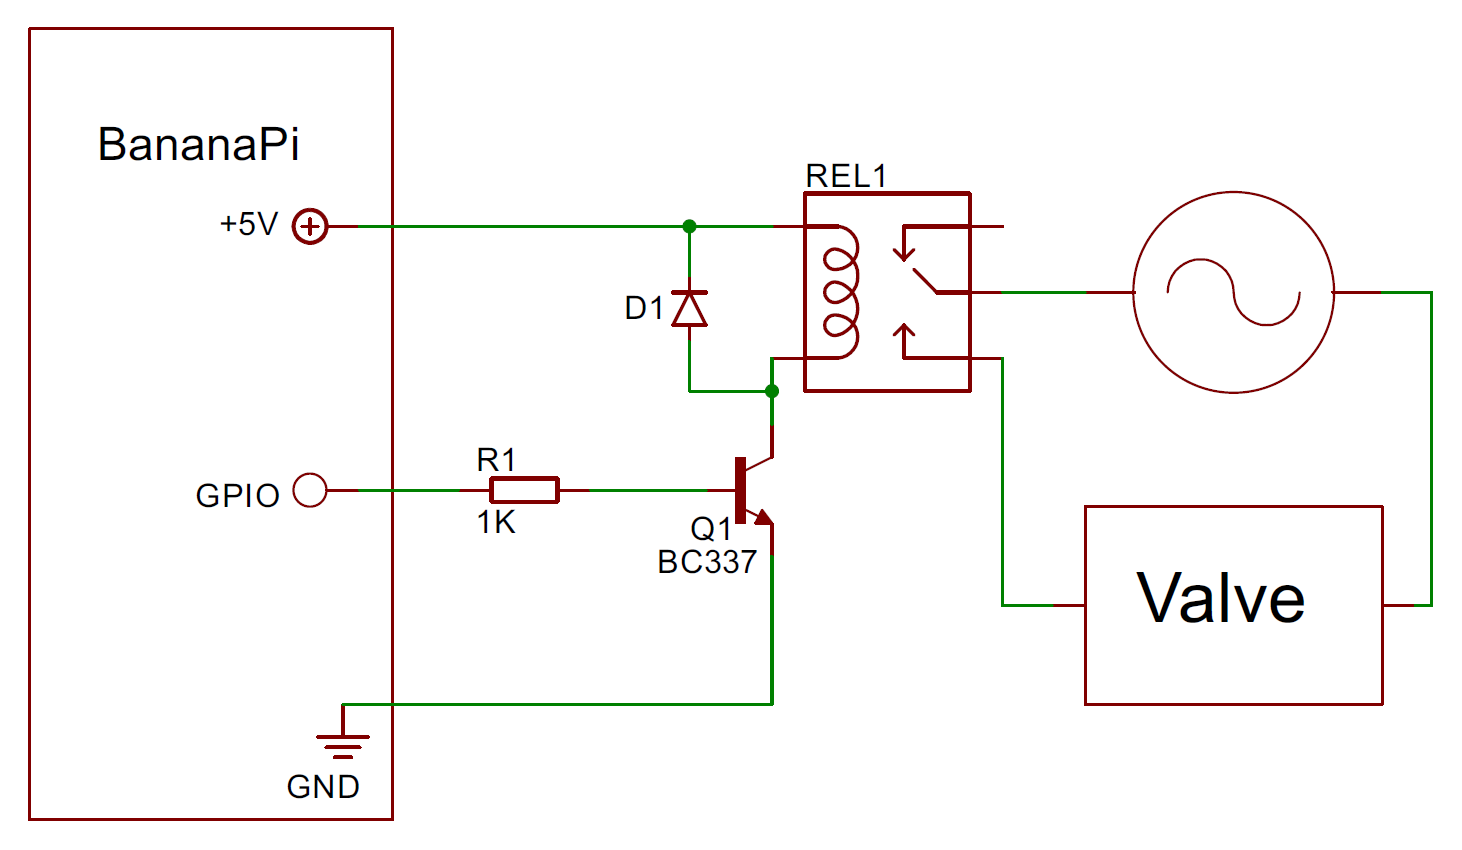
\includegraphics[width=0.95\textwidth]{ControlSchematic}
  \end{center}
  \caption{Heat valve control schematic}
\end{figure}

The standard command line gpio utility built into the Banana Pi is used to control the GPIO pin in the following way:
\lstset{language=PHP}
\begin{lstlisting}[caption={Controlling GPIO in PHP}]
// Switching on the heater
shell_exec('/usr/local/bin/gpio write [gpio pin] 0');

// Switching off the heater
shell_exec('/usr/local/bin/gpio write [gpio pin] 1');
\end{lstlisting}

\chapter{Layout} \label{chap:layout}
The WTherm runs a web interface for user interaction. This chapter will depict how the layout for this user interface was assembled together.
\section{HTML and CSS}
Bootstrap\footnote{\url{http://getbootstrap.com/}} is an open source front-end framework designed to make web-development a lot faster and easier. Bootstrap's CSS framework was used for the WTherm's web interface.
\section{Template parser} \label{sec:TemplateParser}
By using a template parser, a single HTML file with placeholders can be used for every page. This makes editing easier, and it makes the code appear more organized. A simplified version of the template used for the WTherm looks as follows:
\lstset{language=HTML}
\begin{lstlisting}[caption={simplified HTML template},label={lst:htmltemplate}]
<!DOCTYPE HTML>
<html lang="en">
<head>
	<title>WTherm &bull; <?=$this->name?></title>
	<link href="layout/bootstrap.min.css" rel="stylesheet">
	<link href="layout/layout.css" rel="stylesheet">
</head>
<body>
	<?=$PAGE_BODY?>
</body>
</html>
\end{lstlisting}
Notice that the HTML title, menu and body have been replaced by PHP tags. These tags are later replaced by calling the template parser class:
\lstset{language=PHP}
\begin{lstlisting}[caption={Usage of the template parser class},label={lst:templateparser}]
<?php
include('base.php');

$page = new Layout; // Start new layout
$page->startHTML("Home"); // Indicate that HTML code is following
?>

<img src="test.png">

<?php
$HTML = $page->fetchHTML(); // Fetch the above HTML
$page->output($HTML); // Output the layout
?>
\end{lstlisting}
The example above outputs the template, with "Home" in the title tag and the image $test.png$ in the page body.

\chapter{Code overview} \label{chap:codeOverview}
Since the total line count for the software is over 1700, it was not included in this document. The final code can be found in the GitHub repository listed on page~\pageref{chap:Software}. 

In this chapter, the functions of the various scripts are explained. The code is split up into a "Back end" (everything in the $code$ folder except the $www$ folder) and a "Front end" (everything in the $www$ subfolder). The following diagram is an overview of the code structure.
\begin{figure}[H]
  \begin{center}
      \includegraphics[width=0.95\textwidth]{Overview}
  \end{center}
  \caption{Code structure overview}
\end{figure}
\section{Back end}
Back end source code is inaccessible to users. The source code described in this section runs the low-level functions of the thermostat.
\subsection*{base.php}
This file contains global functions, classes as well as configuration variables. This includes the template parser class described in section~\ref{sec:TemplateParser}, the class that calculates the time it will take to heat up to a certain temperature based on the thermal model and a class that handles database connections. $base.php$ is included in nearly every script.
\subsection*{thermostat.php}
This script performs the measurements and controls the heater. Its function is described in the following flowchart:
\begin{figure}[H]
  \begin{center}
      \includegraphics[width=\textwidth,height=0.7\textheight,keepaspectratio]{{thermostat.php}.pdf}
  \end{center}
  \caption{Overview of $thermostat.php$}
\end{figure}

\subsection*{adduser.php and deluser.php}
These scripts can be used to add or delete a user through the command line. Command line usage of $adduser.php$ is as follows:
\lstset{language=bash}
\begin{lstlisting}[caption={Usage of $adduser.php$}]
php5 adduser.php [username] [pass]
\end{lstlisting}
Deleting a user through $deluser.php$ is done in the following manner:
\lstset{language=bash}
\begin{lstlisting}[caption={Usage of $deluser.php$}]
php5 deluser.php [username]
\end{lstlisting}

\subsection*{startup.php}
This script is executed on startup and is used to switch off the heater for the safety concerns discussed in the next chapter.

\section{Front end}
The front end consists of every page that is user-accessible.
\subsection*{JavaScript}
JavaScript, a programming language that is executed client-side, is used to communicate with the database through a technique called AJAX\footnote{Asynchronous JavaScript And XML}. The JavaScript code requests data on the background (\textit{asynchronously}) and uses the response to update the page. This means that the page doesn't have to keep refreshing to update, resulting in a better user experience. This technique is also used for user input. A JavaScript function is triggered when the user interacts with the web page, and updates the database through a PHP file.

\subsection*{login.php}
\begin{figure}[H]
  \begin{center}
      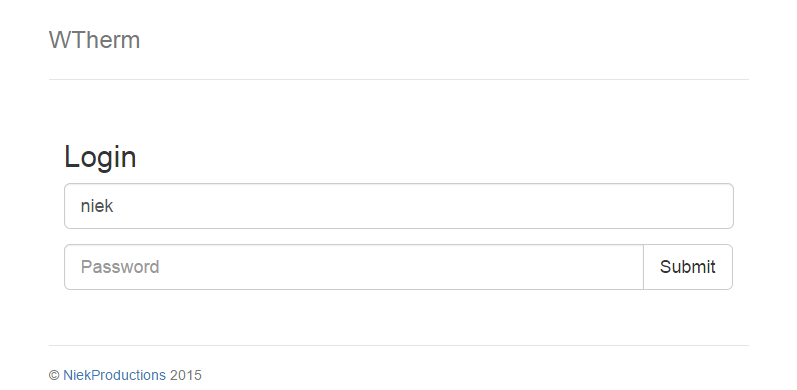
\includegraphics[width=0.95\textwidth]{ui/login}
  \end{center}
  \caption{Preview of the login page}
\end{figure}
This page includes the login form. When this form is submitted, the login is validated. If the username/password combination matches with a username and password hash from the login table in the database the session is registered and the user is redirected to $index.php$. This page is also used to log out, by opening $login.php?logout$.

\subsection*{index.php}
\begin{figure}[H]
  \begin{center}
      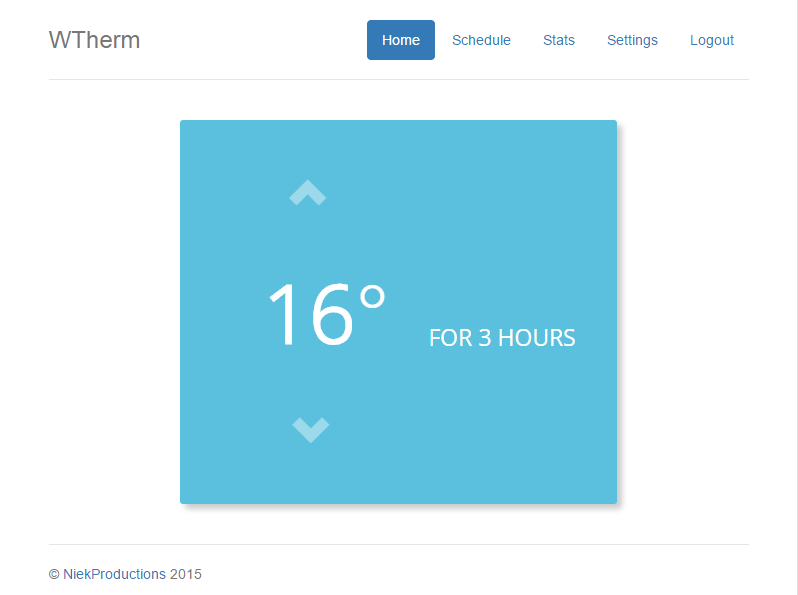
\includegraphics[width=0.95\textwidth]{ui/index}
  \end{center}
  \caption{Preview of the main page}
\end{figure}
This is the main page, where the user can view the target temperature. If the temperature hasn't reached this target yet, the blue square will turn red and the time it will take to heat up will be displayed. Otherwise, the time until the next setpoint according to the schedule will be displayed. This page can also be used to set an override temperature. The override is enabled when the user presses one of the arrows above and below the target temperature. The thermostat will then regulate that temperature until the temperature is pressed. At that point, the thermostat will return to the regular schedule.
\paragraph{control.js} is a JavaScript file included in $index.php$. It handles user communication with the database. For example, when the page loads, $control.js$ requests the target temperature and override status from $data.php$ which in turn communicates with the database. $control.js$ also interacts with $data.php$ to set a temporary target temperature in the database.

\subsection*{schedule.php}
\begin{figure}[H]
  \begin{center}
      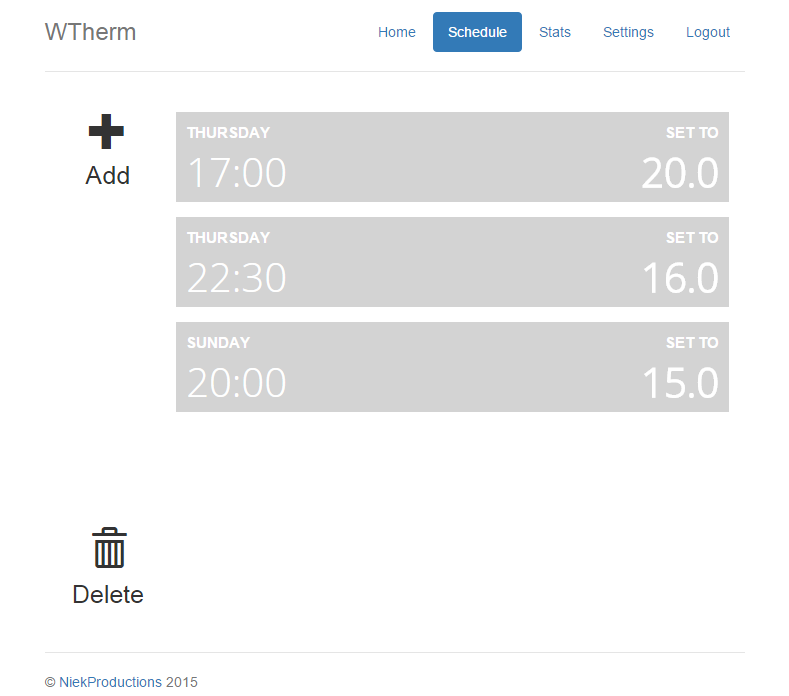
\includegraphics[width=0.95\textwidth]{ui/schedule}
  \end{center}
  \caption{Preview of the schedule}
\end{figure}
This page is used to set the schedule. The schedule consists of targets (or setpoints) that can be added by clicking the $Add$ button on the left of the page. If a setpoint is selected by clicking on it, it will turn blue and be editable. A setpoint can be deleted using the $Delete$ button.

\paragraph{schedule.js} is used in $schedule.php$ to edit and save the setpoints. The $Add$ and $Delete$ buttons trigger JavaScript functions that interact with the setpoint. After every edit, JavaScript passes the array of SetPoints onto $schedule.php$ to be saved to the database. After every edit, the schedule is saved.

\subsection*{stats.php}
\begin{figure}[H]
  \begin{center}
      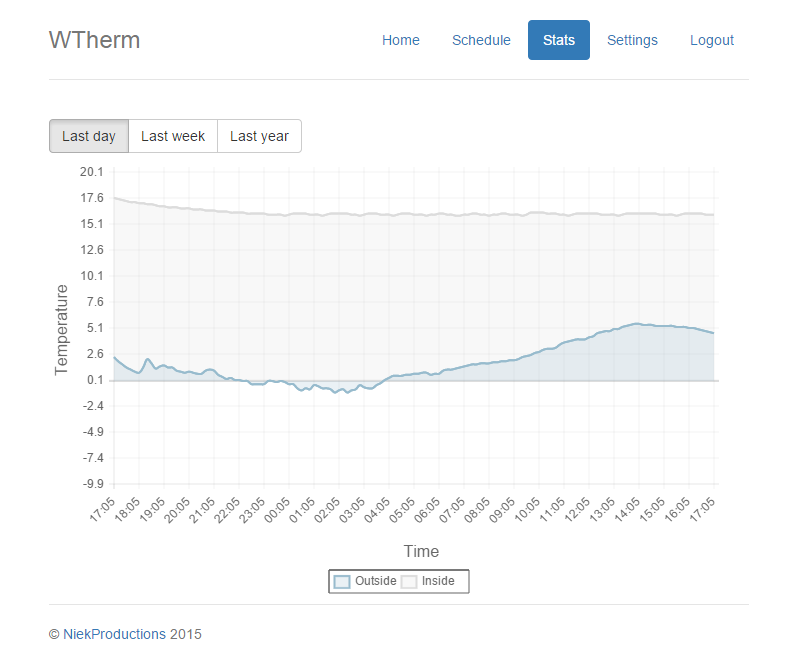
\includegraphics[width=0.95\textwidth]{ui/stats}
  \end{center}
  \caption{Preview of the statistics page}
\end{figure}
This page contains charts of the inside and outside temperature over the period of a day, a week or a year. It uses the JavaScript ChartNew.js library\footnote{\url{https://github.com/FVANCOP/ChartNew.js/}} to draw the charts.

\paragraph{drawChart.js} is used to specify options for the chart. It uses AJAX to obtain the contents of the log database table through $chartdata.php$.

\subsection*{settings.php}
\begin{figure}[H]
  \begin{center}
      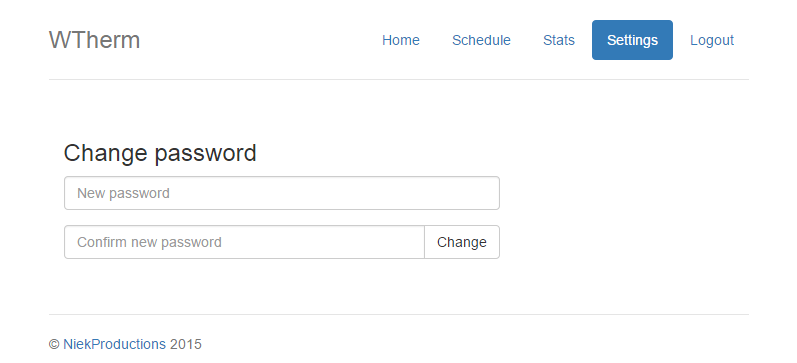
\includegraphics[width=0.95\textwidth]{ui/settings}
  \end{center}
  \caption{Preview of the settings page}
\end{figure}
The settings page allows a user to change their password. 

\chapter{Safety features} \label{chap:safety}
In the previous chapter, the function of every source code file was described. This chapter will cover the safety features that were implemented.
\section{Dealing with reboots}
If the thermostat ever loses power, the heater is automatically switched off since the relay described in chapter~\ref{chap:heaterInterface} is normally-open, meaning it will disconnect the heating valve's power if it's not powered.

On the software side, a script is run on reboot that switches the heater off in the case of a power loss.

\section{Script freezes}
If the $thermostat.php$ script ever freezes, it will not give rise to a safety concern, since the script is automatically restarted every five minutes.

\section{Preventing unreliable measurements}
The thermostat might be unable to request the temperature from the HomeWizard. To prevent this causing issues, the heater will be switched off in case no temperature measurements can be obtained for a subsequent period of 10 minutes. This prevents the heater from switching on when the temperature might already have exceeded the target.

\part{Calculating energy savings} \label{part:CalculateSavings}
Now that the source code has been explained, the next step is to find out if the WTherm can actually save a significant amount of energy. This is done by comparing the WTherm to a traditional clock thermostat over the course of a single week in the winter.

Imagine a situation in which a household would like the temperature to be 20\degree{}C at 9:00 every morning. They set a traditional clock thermostat to start heating at 6:30. Assuming a constant starting temperature of 18\degree{}C, the heating time was calculated for an entire week in December 2014. Outside temperatures were used from the weather archive of the Royal Netherlands Meteorological Institute (KNMI)\footnote{\url{http://www.knmi.nl/klimatologie/uurgegevens/}}:
\begin{figure}[H]
  \begin{center}
      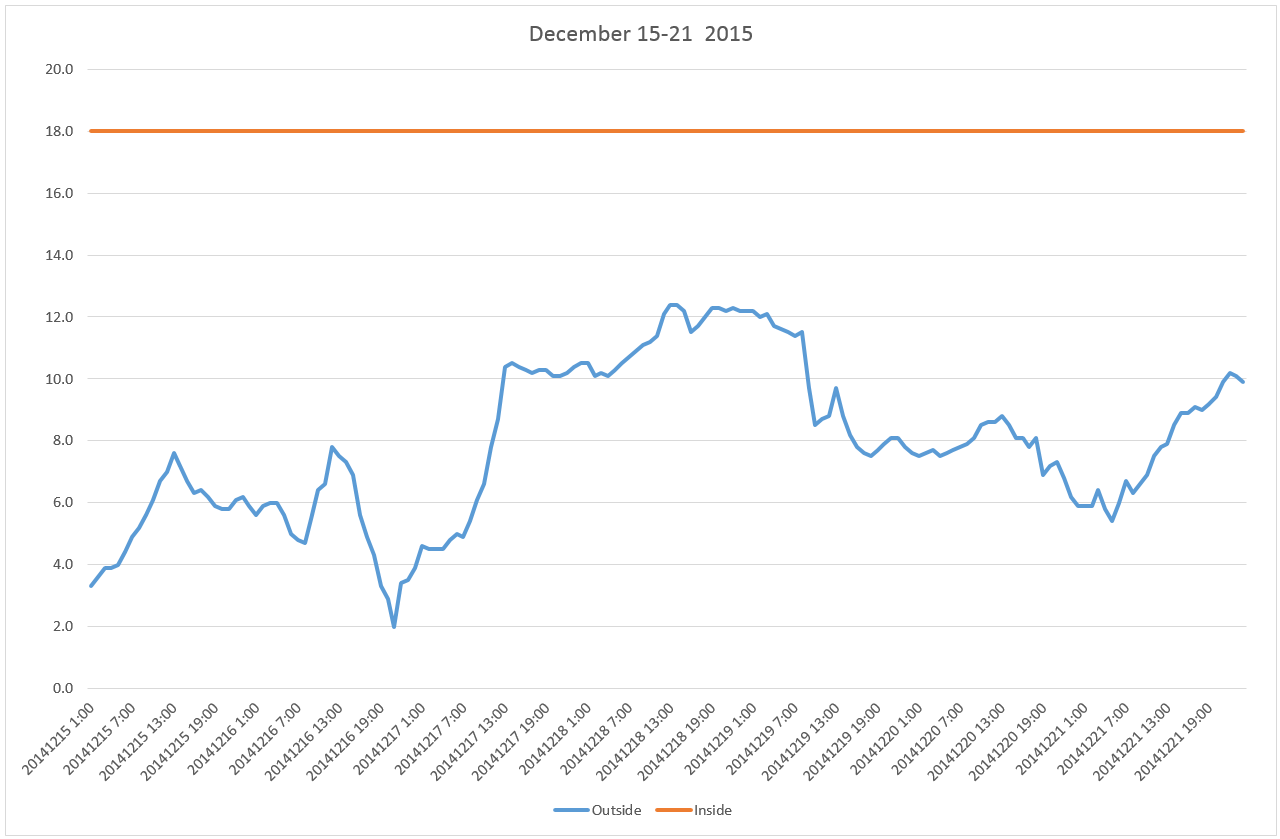
\includegraphics[width=0.95\textwidth]{EnergySavings-compare}
  \end{center}
\end{figure}

Based on the thermal model from page~\pageref{sec:usingModel}, it can be calculated that the guess above is almost correct for the first day. The outside temperature was 5.0\degree{}C and it would take 2.6 hours to heat up to 20\degree{}C. The same goes for the second and third day, with a heating time close to 2 and a half hours.

The fourth day however, the outside temperature reached a significantly higher number and it would have taken just over an hour to heat up to 20\degree{}C. This means that the thermostat spent an additional one and a half hours keeping the temperature at 20\degree{}C, at the cost of a significant amount of heat. An overview for the entire week is listed in the table below:

\begingroup
	\setlength{\LTleft}{-20cm plus -1fill}
	\setlength{\LTright}{\LTleft}
    \begin{longtable}{ | p{1.0cm} | p{3cm} | p{3cm} | p{3cm} | p{2cm} |}
    \hline
    Day & Outside temperature (\degree{}C) & Human guess (hours) & Actual heating time (hours) & Difference (hours) \\ 
    \hline
    1 & 4.7 & 2.5 & 2.6 & -0.1\\ 
    \hline
    2 & 4.9 & 2.5 & 2.5 & 0\\
    \hline
    3 & 5.0 & 2.5 & 2.4 & +0.1\\
    \hline
    4 & 10.8 & 2.5 & 1.2 & +1.3\\
    \hline
    5 & 11.5 & 2.5 & 1.1 & +1.4\\
    \hline
    6 & 7.8 & 2.5 & 1.6 & +0.9\\
    \hline
    7 & 6.5 & 2.5 & 1.9 & +0.6\\
    \hline 
    \end{longtable}
    \captionof{table}{Heating time overview}
\endgroup


This table shows that the traditional thermostat would have spent an additional total of 4.2 hours keeping the temperature at 20\degree{}C. Using the outside temperatures and the heat transfer coefficient from~\ref{sec:CalculatePUC}, it can be calculated that during these 4.2 hours, 15.6kWh has been used in order to maintain a constant room temperature. Assuming the WTherm to have switched on the heater at exactly the right time, it would have saved exactly this amount of energy. 

According to the KNMI, the winter of 2014-2015 lasts for three months, or about 
13 weeks \cite{KNMIseizoensdata}. If all of those weeks would be similar to the one described here, a total amount of 731 megajoules of heat could have been saved

The Dutch energy supplier Nuon employs a maximum rate of \EUR{22,64} per GJ for district heating\cite{NuonStadsverwarming}. This amounts to yearly savings of \EUR{16,56}.

The same energy supplier charges \EUR{0,64} per $\mathrm{m^{3}}$ of natural gas\cite{NuonGas}. The heating value of natural gas from the Netherlands is $\mathrm{32\times 10^{6} Jm^{-3}}$ \cite{BinasHeatingValue}, meaning that the same 0,73 gigajoules would cost \EUR{14,62}.

In this situation, over \EUR{16} can possibly be saved every winter, which is over one third the total cost of the used materials listed in the bill of materials on page~\pageref{chap:BOM}.

\part{Conclusion}
The objective of this research was to develop a smart web-based thermostat, WTherm, that saves energy by calculating the time it takes to heat up a living room to a certain temperature. The smart thermostat uses this calculation to precisely follow a weekly schedule that can be programmed through a web-interface. The calculation is based on a thermal model that incorporates several formulas. This thermal model is used to switch the heater on at the right time, reducing the total heater-on time.

Temperatures over the course of a week during the winter were used to compare the WTherm to a traditional room thermostat. The hypothesis was proven that, in comparison with a traditional room thermostat, a considerable amount of energy can be saved. In this specific situation, \EUR{16,50} can be saved every year. This is a third of the cost of the materials used, thus proving that the WTherm will pay for itself in three years. This also indicates that the WTherm is a more cost-efficient replacement for a traditional clock thermostat.

\part{Discussion}
The results might be arguable for a number of reasons.

First of all, the thermal model is based on measurements performed in a room that wasn't heated for a couple of days, meaning that every object in the room also had to be heated up. To verify if the same model could apply to a situation in which the room has been heated the previous day, the traditional room thermostat was set to heat up to 19,5\degree{}C at 7:20. This temperature was reached 50 minutes later. The starting temperature was 18,6\degree{}C and the average outside temperature was 3,35\degree{}C. According to the model, the goal temperature should have been reached after one and a half hours, which is incorrect.

Secondly, the model was created with a relatively high outside temperature. This means that if the difference between inside and outside temperatures is over 19.7\degree{}C, $Qloss$ is higher than $Qin$ and the room will not heat up at all according to the model. In reality, this is not the case. Many variables were assumed constant. The heating power for example depends on external influences such as inside and outside air humidity. If the sun is shining through the windows the room will also heat up in a smaller amount of time.

The two issues addressed above can be solved by creating different thermal models for various inside and outside temperatures. Ideally, this could be done automatically using the automatic heat meter readout described in the next chapter.

Furthermore, the calculated savings might not be entirely accurate. The yearly cost reduction of the energy bill was based on calculated savings for an entire week which were extrapolated to an entire winter. The actual amount of preserved energy might vary from week to week. In addition, only the duration of the meteorological winter was used in this calculation. A larger amount of energy could be saved if the room is also heated during the autumn or spring. This signifies that the WTherm will most likely have paid for itself within the calculated three years.

Another possible concern relates to the heater, which is only turned off when the target temperature has been reached. This can cause an overshoot in temperature, since there's a delay between switching the heater on and a temperature rise being measured. A simple solution might be to switch off the heater a couple of tenths of degrees below the target temperature to account for the overshoot, but this constant offset won't be very accurate as the overshoot depends on external factors. This also might result in rapid heater toggling, as the temperature fluctuates around the target. A better solution would be to use a PID\footnote{Proportional-Integral-Derivative} loop. A PID loop would control the heating by calculating Proportional, Integral and Derivative responses and summing those three components to compute the output\cite{PIDexplained}. A PID based thermostat eliminates temperature overshoot.


\chapter{Possible future research}
\section{Automatic heat meter readout}
According to the Landis \& Gyr catalog sheet, the heat meter installed in this household has got several ways of retrieving the exchanged heat\cite{landisgyrcat14}. One of the ways described is through an IR\footnote{Infrared} interface. Landis \& Gyr has published a specification sheet\cite{landisgyrser14} detailing the protocol. Obtaining the added heat over the IR interface can be done using an optical read-out head\footnote{\url{http://www.multical.hu/Optical_Read-out_Head_datasheet.pdf}}. If this transceiver would be connected to the WTherm, it could autonomously create and improve thermal profiles. This would also simplify integration of the WTherm into other households since the read-out head is IEC 1107/EN 61107 compliant, meaning that it will work with other heat meters that support this standard.

\section{Reliable heat measurements}
The inside and outside temperatures are currently obtained through two wireless sensors. These sensors can only be read in the accuracy range of a single decimal number and occasionally need a replacement battery. To eliminate batteries and increase the accuracy, a high-precision wired digital thermometer such as the NXP SE95\footnote{\url{http://www.nxp.com/documents/data_sheet/SE95.pdf}} can be used. This sensor has a resolution of 0,03125\degree{}C.

\section{User presence detection}
A possibility to save more energy would be to automatically switch off the heater when no user is present in the house. This could be detected by scanning for the presence of smartphones on the network. If all smartphones disappear, the WTherm can switch off the heater on the presumption that nobody is in the house. Once a user enters the house and their smartphone automatically connects to the wireless network, the WTherm can automatically switch the heater back on.

\section{Compatibility with other households}
At the moment, the thermostat is only installed in a single situation. It can only be used in comparable households with a heat meter. Using the automatic heat meter readout described in the first section of this chapter, the WTherm could be installed in other households. A future research might explore this possibility.
\newpage
\printbibliography
\vfill

\part*{Appendix}
\phantomsection
\addcontentsline{toc}{part}{Appendix}
\chapter{License} \label{chap:License}
This work is licensed under the Creative Commons Attribution-NonCommercial-ShareAlike 4.0 International License. To view a copy of this license, visit \url{http://creativecommons.org/licenses/by-nc-sa/4.0/}.
\begin{figure}[H]
  \begin{center}
      
\includegraphics{by-nc-sa}
  \end{center}
\end{figure}

\chapter{Software} \label{chap:Software}
All of the code for this project is available on GitHub at \url{https://github.com/NiekProductions/WTherm/}. Unlike this document, it was released under the MIT License. This is a permissive license, meaning that people can do anything they'd like with the code as long as they provide attribution to the original source. It also excludes every liability. A full copy of the license is available in the $LICENSE$ file on GitHub.

\chapter{Demo}
A non-functional demo of the web interface used for the WTherm is available at \url{http://niekproductions.com/wtherm/}.

\chapter{Git}
To store code and keep track of changes Git\footnote{\url{http://git-scm.com/}} was used. Git is version control software that stores the contents of a directory as sequential snapshots. In this project, it was used to keep track of file differences in this document and the source code.

\chapter{\LaTeX}
A word processor like Microsoft Word could have been used to write this thesis, but it comes with several disadvantages. Mostly, it’s hard to manage a document in the format that Word uses. Version control software like Git can only handle the file in a binary format, meaning that differences between versions are not visible.

Instead of Word, \LaTeX{}\footnote{\url{http://www.latex-project.org/}} was used to write this thesis. \LaTeX{} is a mark-up language, much like HTML. It was explicitly designed for writing large scientific papers, and saves documents in plain text making them easy to read. \LaTeX{} supports packages that make it easy to insert chunks of code and reformat the document.

\chapter{Bill of materials} \label{chap:BOM}
\begin{tabular}[c]{l c c r}
	Part & Price & Amount & Total price \\
	\hline
	Banana Pi & \EUR{39,99} & 1 & \EUR{39,99} \\
	Relay, transistor, passive components & \EUR{1,50} & 1 & \EUR{1,50} \\
	\\ & & Total: & \EUR{41,49} \\
\end{tabular}
\captionof{table}{Bill of materials}

\chapter{Installation instructions}
Installation instructions can be found in the $README$ file on GitHub using the link provided in chapter~\ref{chap:Software}.

\newpage
\chapter{Log}
\begingroup
	\setlength{\LTleft}{-20cm plus -1fill}
	\setlength{\LTright}{\LTleft}
    \begin{longtable}{ | p{2.5cm} | p{2.5cm} | p{5cm} | p{2cm} |}
    \hline
    Date & Location & Activity & Duration \\ 
    \hline
    30-04-2014 to 07-07-2014 & Home & Preliminary research - WTherm alpha & 30 hours (estimated) \\ 
    \hline 
    18-09-2014 & Home & Finding a subject, outlining idea, brainstorming & 1:00 \\ 
    \hline
    09-11-2014 & Hackerspace & Brainstorming, outlining research question & 2:00 \\
    \hline
    10-11-2014 & Home & Started writing research proposal & 1:00 \\
	\hline
	11-11-2014 & Home & Continued working on research proposal & 1:30 \\
	\hline
	12-11-2014 & Home & Continued working on research proposal & 0:45	\\
	\hline
	18-11-2014 & School & Finished research proposal & 2:20	\\
	\hline
	25-11-2014 & School & Familiarizing with \LaTeX, setting up Git, starting first chapter & 2:20 \\
	\hline
	27-11-2014 & School & Continued writing first chapter in \LaTeX , started bibliography & 1:20 \\
	\hline
	29-11-2014 & Home & Worked on document formatting, moved the log to the document. Continued chapter one. & 3:15 \\
	\hline
	30-11-2014 & Home & Continued working on chapter one & 1:30 \\
	\hline
	01-12-2014 & Home & Started hardware choice chapter & 0:30 \\
	\hline
	02-12-2014 & School & Researched radiated heat and heat transfer & 2:20 \\
	\hline
	05-12-2014 & Home & Researched how to interface with heat meter, planned measurements, started converting bibliography to Bib\LaTeX{} & 2:30 \\
	\hline
	06-12-2014 & Home & Performed test measurement for thermal model, continued converting bibliography to Bib\LaTeX{} & 3:30 \\
	\hline
	07-12-2014 & Home & Researching modeling in physics, finished converting bibliography to Bib\LaTeX{} & 1:30 \\
	\hline
	09-12-2014 & School & Started a thermal model of the room & 2:20 \\
	\hline
	11-12-2014 & School & Processing measurements, planned new measurements & 1:30 \\
	\hline
	12-12-2014 & Home & Set up camera for measurements & 0:30 \\
	\hline
	13-12-2014 & Home & Performing measurements & 2:00 \\
	\hline
	14-12-2014 & Home & Processing measurements & 3:00  \\
	\hline
	16-12-2014 & School & Continued processing measurements & 2:20 \\
	\hline
	17-12-2014 & Hackerspace & Tried to compose a formula describing the heating time, documenting & 3:00 \\
	\hline
	18-12-2014 & School & Drafted thermal model of the living room & 1:30 \\
	\hline
	21-12-2014 & Hackerspace & Corrected thermal model & 1:00 \\
	\hline
	24-12-2014 & Home & Finished description of equations & 1:45 \\
	\hline
	26-12-2014 & Home & Processing measurements for thermal model & 6:45 \\
	\hline
	27-12-2014 & Home & Finished thermal model, documenting & 8:00 \\
	\hline
	28-12-2014 & Hackerspace & Started part 2, researched programming languages and webservers & 5:00 \\
	\hline
	01-01-2015 & Home & Set up control measurement & 1:00 \\
	\hline
	03-01-2015 & Home & Started writing code, set up new measurement & 7:45 \\
	\hline
	04-01-2015 & Hackerspace & Continued writing code, working on discussion, rewriting first chapter & 4:00 \\
	\hline
	06-01-2015 & School & Documenting MySQL login code and password hashing & 2:20 \\
	\hline
	11-01-2015 & Home & Writing code. Finished schedule, database class, template parser and login system & 10:30 \\
	\hline
	12-01-2015 & Home & Setting up Banana Pi, installing LEMP stack & 2:30 \\
	\hline
	13-01-2015 & School & Writing code, working on thermCalc class & 2:00 \\
	\hline
	14-01-2015 & Home & Writing thermostat code & 2:30 \\
	\hline
	16-01-2015 & Home & Writing code, finished thermostat script, mostly finished user interface & 10:15 \\
	\hline
	17-01-2015 & Home & Installing thermostat, configuring git, writing chart page & 6:30 \\
	\hline
	18-01-2015 & Hackerspace & Reviewing chapters, formatting & 5:00 \\
	\hline
	19-01-2015 & Home & Writing introduction & 1:00 \\
	\hline
	21-01-2015 & Home & Continued writing introduction, revising first chapter & 4:00 \\
	\hline
	24-01-2015 & Home & Calculated energy savings & 4:15 \\
	\hline
	25-01-2015 & Hackerspace & Creating diagrams, re-reading and rewriting large parts & 6:45 \\
	\hline
	26-01-2015 & Home & Proofreading and rewriting parts & 2:00 \\
	\hline
	27-01-2015 & Home & Finishing I-2 & 4:45\\
	\hline
	28-01-2015 & Hackerspace & Rewriting, writing code overview & 4:15 \\
	\hline
	29-01-2015 & Home & Finishing code overview, introduction, conclusion & 8:45 \\
	\hline 
	05-02-2015 & School & Rewriting sections, correcting calculations & 2:45\\
	\hline
	& & Total (excluding preliminary research) & 158 hours\\
	\hline
    \end{longtable}
    \captionof{table}{Log}
\endgroup

\listoffigures
\listoftables
\end{document}